%% LyX 2.0.3 created this file.  For more info, see http://www.lyx.org/.
%% Do not edit unless you really know what you are doing.
\documentclass[twoside,english]{elsarticle}
\usepackage[T1]{fontenc}
\usepackage[latin9]{inputenc}
\pagestyle{headings}
\setlength{\parskip}{\smallskipamount}
\setlength{\parindent}{0pt}
\usepackage{verbatim}
\usepackage{graphicx}

\makeatletter
%%%%%%%%%%%%%%%%%%%%%%%%%%%%%% User specified LaTeX commands.
% specify here the journal
\journal{}

% use this if you need line numbers
%\usepackage{lineno}

\makeatother

\usepackage{babel}
\begin{document}





\title{Predictive Quality Control}


\author[rvt]{C.V.~Radhakrishnan\fnref{fn1}\corref{cor1}\corref{cor2}}


\ead{cvr@river-valley.com}


\author[rvt,focal]{K.~Bazargan\fnref{fn2}}


\ead[url]{http://www.elsevier.com}


\fntext[fn1]{This is the specimen author footnote.}


\fntext[fn2]{Another author footnote, but a little more longer.}


\cortext[cor1]{Corresponding author}


\cortext[cor2]{Principal corresponding author}


\address[rvt]{River Valley Technologies, SJP Building, Cotton Hills, Trivandrum,
Kerala, India 695014}


\address[focal]{River Valleysfgs Technologies, 9, Browns Court, Kennford, Exeter,
United Kingdom}
\begin{abstract}
Abstract, should normally be not longer than 200 words. All work and
no play makes jack a dull boy. All work and no play makes jack a dull
boy. All work and no play makes jack a dull boy. All work and no play
makes jack a dull boy. All work and no play makes jack a dull boy.
All work and no play makes jack a dull boy. All work and no play makes
jack a dull boy. All work and no play makes jack a dull boy. All work
and no play makes jack a dull boy. All work and no play makes jack
a dull boy. All work and no play makes jack a dull boy. All work and
no play makes jack a dull boy. All work and no play makes jack a dull
boy. All work and no play makes jack a dull boy. All work and no play
makes jack a dull boy. All work and no play makes jack a dull boy.
All work and no play makes jack a dull boy. All work and no play makes
jack a dull boy. All work and no play makes jack a dull boy. All work
and no play makes jack a dull boy. All work and no play makes jack
a dull boy. All work and no play makes jack a dull boy. All work and
no play makes jack a dull boy. All work and no play makes jack a dull
boy. All work and no play makes jack a dull boy. All work and no play
makes jack a dull boy. All work and no play makes jack a dull boy.
All work and no play makes jack a dull boy. All work and no play makes
jack a dull boy. All work and no play makes jack a dull boy. All work
and no play makes jack a dull boy. All work and no play makes jack
a dull boy. All work and no play makes jack a dull boy. All work and
no play makes jack a dull boy. All work and no play makes jack a dull
boy. All work and no play makes jack a dull boy. All work and no play
makes jack a dull boy. All work and no play makes jack a dull boy.
All work and no play makes jack a dull boy. All work and no play makes
jack a dull boy. All work and no play makes jack a dull boy. All work
and no play makes jack a dull boy. All work and no play makes jack
a dull boy. \end{abstract}
\begin{keyword}
quadruple exiton \sep polariton \sep WGM \PACS 71.35.-y \sep 71.35.Lk
\sep 71.36.+c \MSC[2008]23-557
\end{keyword}
\maketitle



\section{Introduction}


\subsection{How is quality measured in present time?}

Present day quality measurements are done using various metrological
tools which quantify various shapes and/or form features of the part.
These features are given their individual limits by the designer which
help a metrologist in determining whether a part that has just been
manufactured is fit to be deemed a good part or not. However, most
of these tools are completely external equipments which need to be
explicitly used over the part(s) to see the results. This usually
calls for extra man-power and reduced throughput. So what manufacturers
end up doing is that they keep an inspection frequency for non critical
parts where quality checks on these parts are made at regular intervals
until one sees an anomaly. How this anomaly is responded to again
depends on what feature we are measuring.

The main problem with such a way of measurement is that :-
\begin{enumerate}
\item We have to make a compromise between the throughput and inspection
interval.
\item As the quality measurement is isolated from part manufacturing, you
can\textquoteright{}t detect a bad part unless it has already been
manufactured.
\end{enumerate}

\subsection{How do we propose to measure it?}

The main gist of the ideology we have applied is that, when a part
is being made, the information of each cut made by the machine is
reflected in some real-time aspect of the machine. It could be noise,
power, vibration, loads, etc. So what we do is, we record these variables
(in our case, power) real-time using appropriate tools and find a
correlation between these readings and the quality of the part manufactured.
This correlation can be tightened depending on the kind of accuracy
one is looking for. It also has an advantage over the conventional
approach in certain key aspects such as:-
\begin{enumerate}
\item The computational time is significantly less once a correlation model
has been made. Also, buying computational time is cheaper than wasting
producing time.
\item The feedback we get is near to real time and we could infact get early
warnings as the part is being made.
\item The kind of investment needed for this is much lesser compared to
buying precise instruments which, other than being pretty expensive,
usually have only a single functionality.
\end{enumerate}

\section{Methodology}


\subsection{Getting Quality data}

As we need to correlate between power readings during a producing
cycle and quality, we are essentially trying to create a model or
create a procedure to generate a model which would take the power
readings as input and give the quality as output. Thus, we needed
some input quality data for a training set.

For this, we monitored the Ra values of a part, which underwent turning
operation, at regular intervals (once in 25 parts for first 500 cycles
and once in every 10 parts from there on) for 1030 parts. These measurements
were made at two different faces and three different locations in
each face. We observed a downward trend in the Ra values for the first
300 parts after which they were more or less constant (no particular
trend) till part 1000 after which they again rose up and went outside
the specification limit.%
\begin{comment}
Should graphs of all six paramaters be drawn?
\end{comment}


So we decided to use the trend evident in the first 300 parts for
our model creation and verification. We created a 2 degree polynomial
fit for the first three hundred parts using 12 readings as our control
points.%
\begin{comment}
INSERT FIGURE AND POLYFIT STATS.
\end{comment}
{} The equation turns out to be 
\begin{equation}
y\approx3.35664-0.00324170.x+0.000006684611.x^{2}\label{eq:polyfit_1}
\end{equation}


Where, $y$ is the Ra value and $x$ is the part number. We see a
maximum error of $0.0833\mu m$ in the fit. For figure, see Fig.\ref{fig:Polynomial-fit-of Ra}
for the curve and Fig.\ref{fig:Residuals-of-polynomial_ra} for the
residuals' curve.

\begin{figure}[!tph]
\noindent \begin{centering}
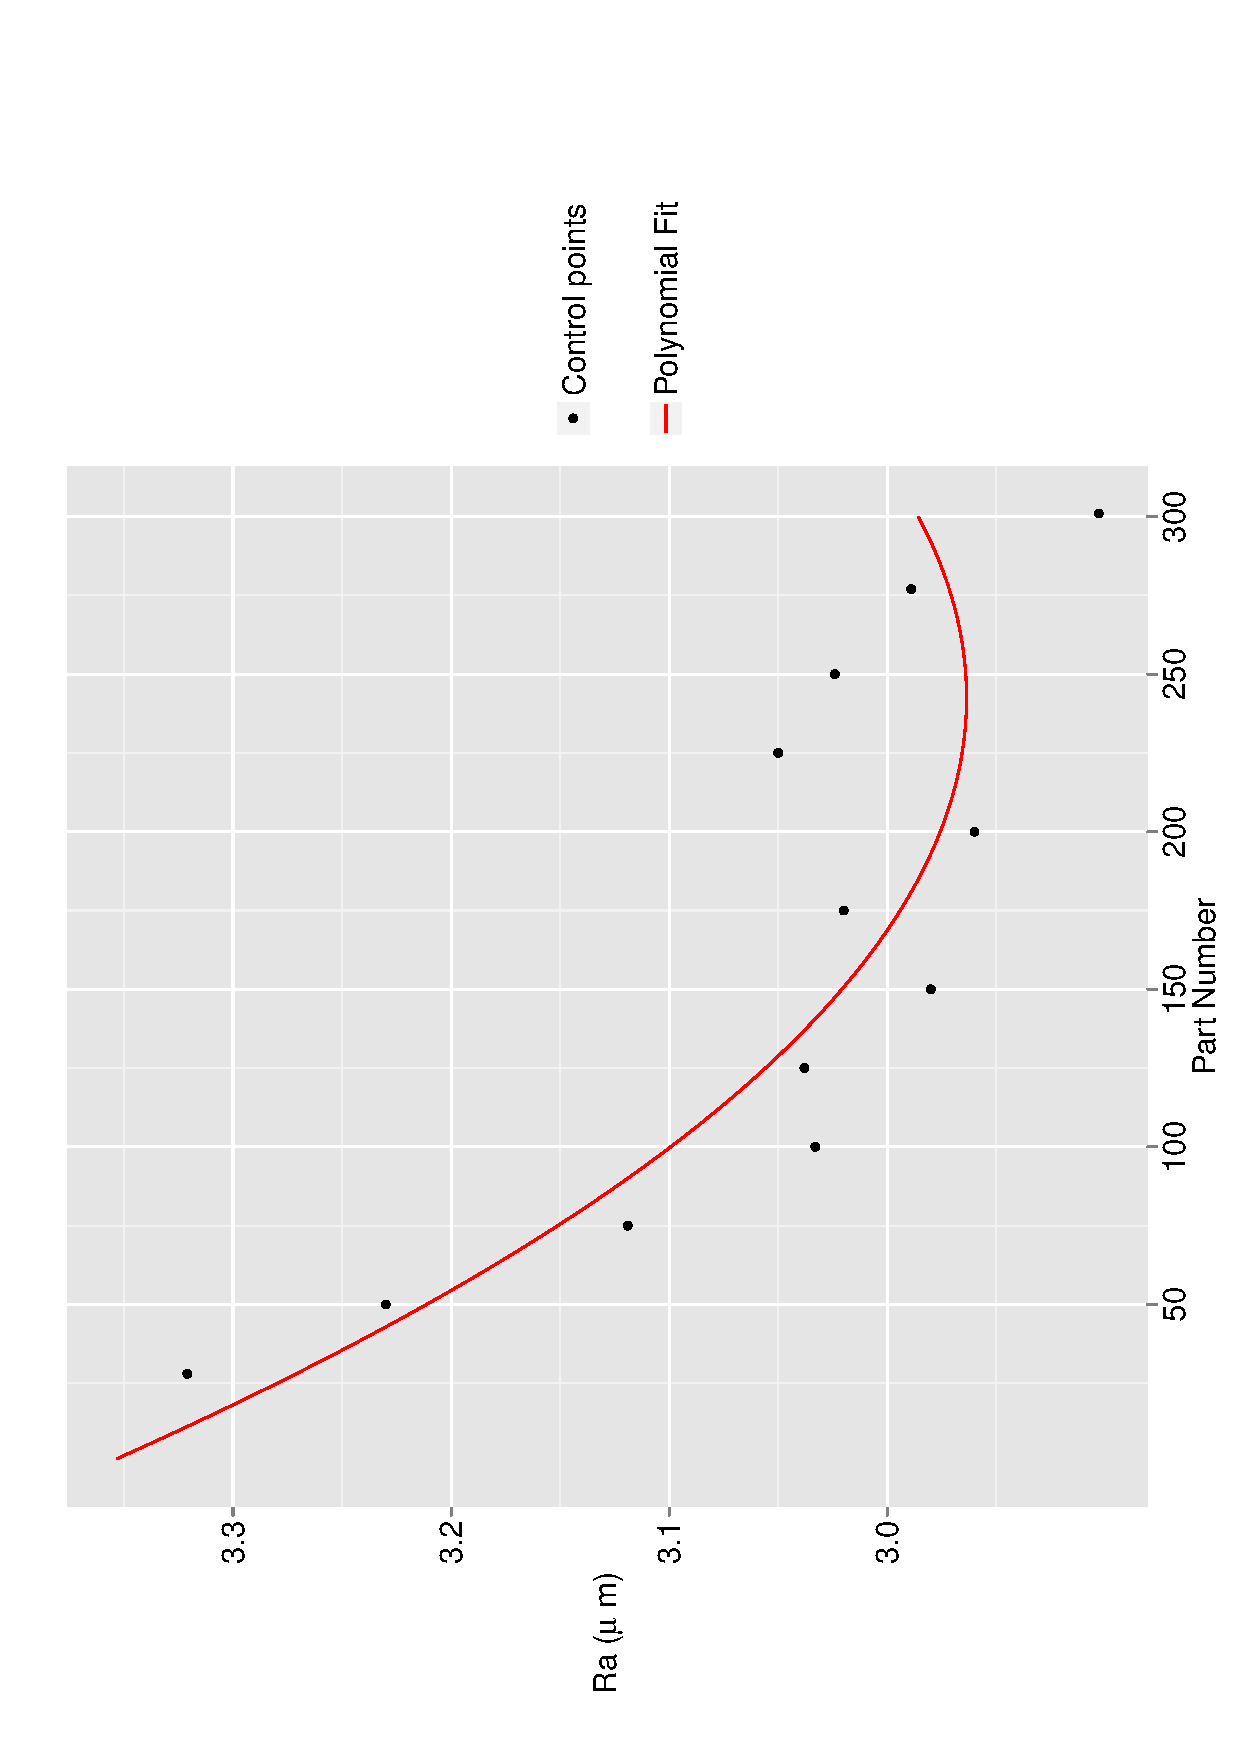
\includegraphics[clip,width=14cm,height=8cm]{Images/poly_fit_Ra}
\par\end{centering}

\noindent \centering{}\caption{Polynomial fit of Ra values\label{fig:Polynomial-fit-of Ra}}
\end{figure}


\begin{figure}[!tph]
\noindent \begin{centering}
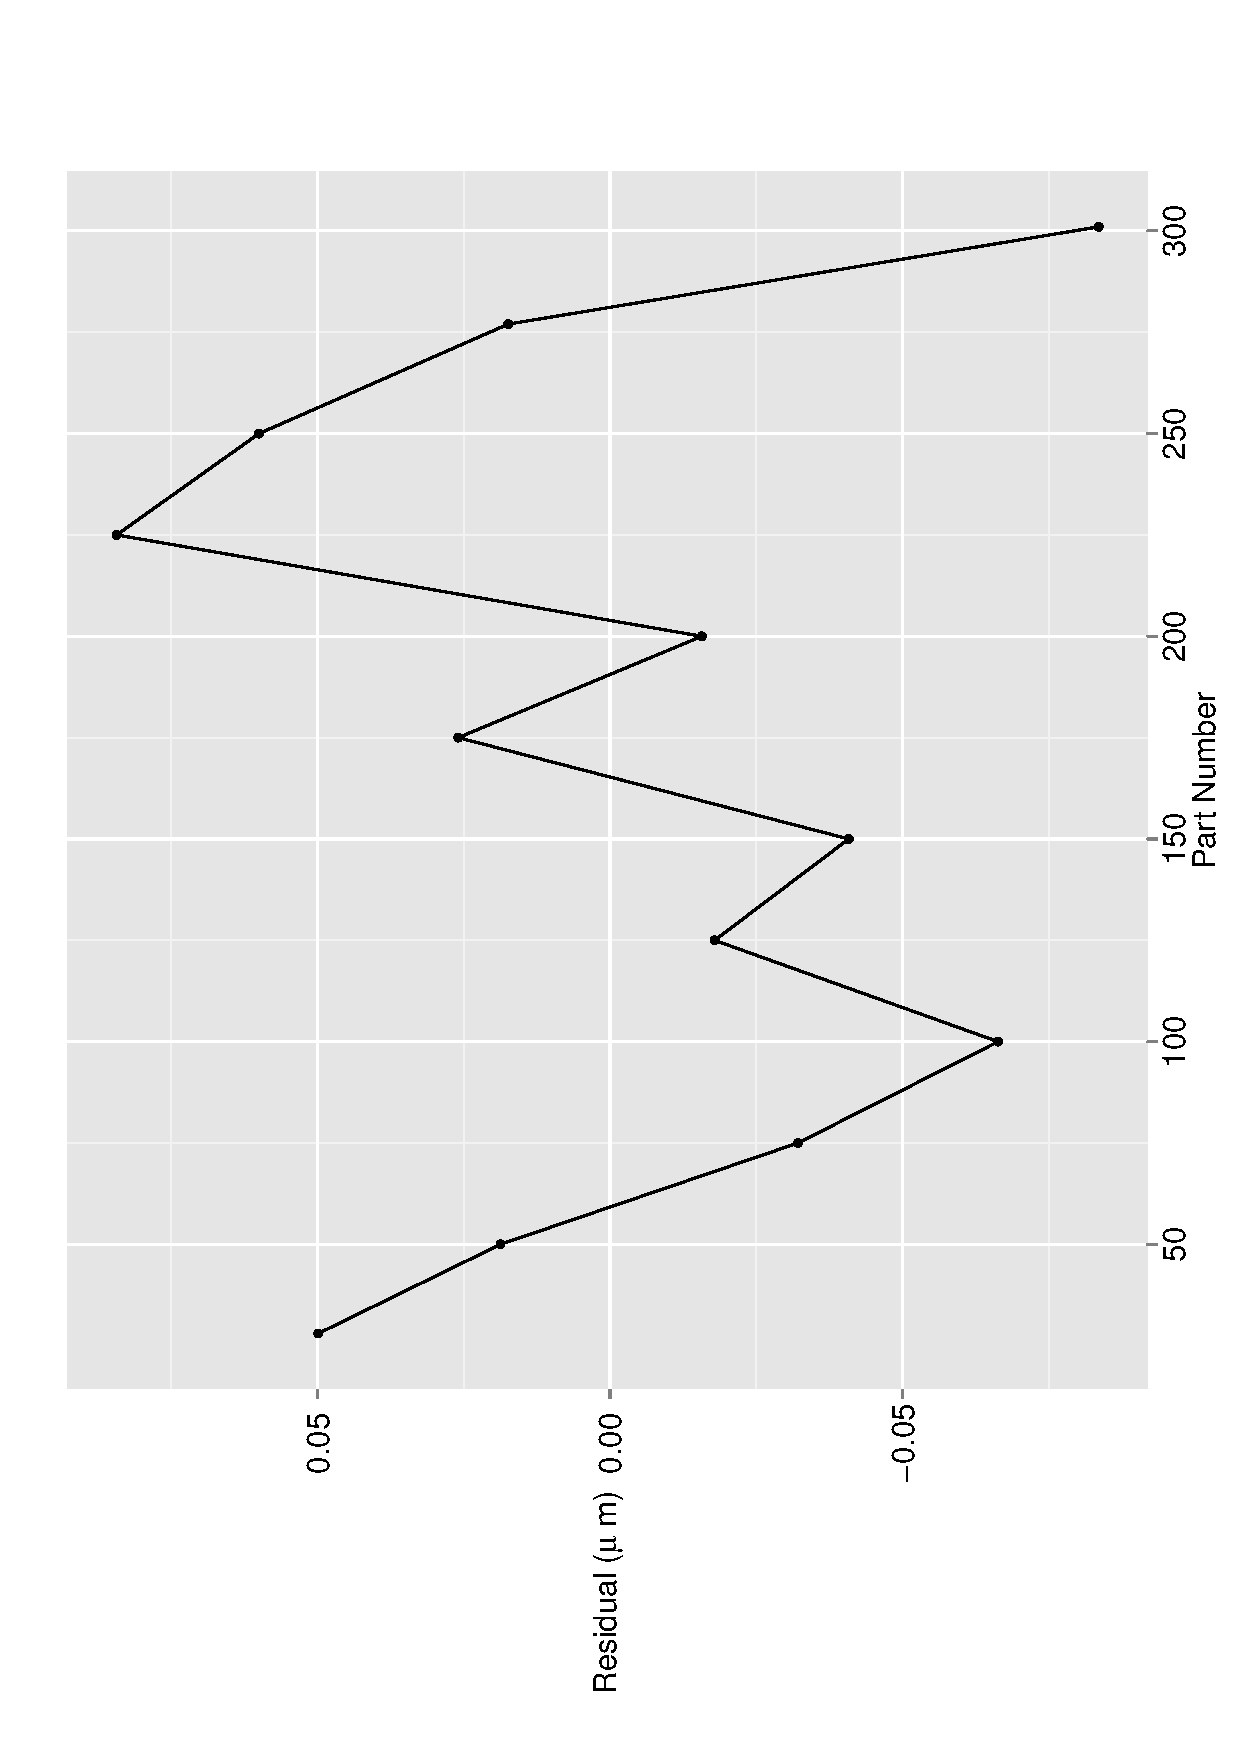
\includegraphics[width=14cm,height=8cm]{Images/poly_fit_residual}
\par\end{centering}

\noindent \begin{centering}
\caption{Residuals of polynomial fit for Ra values\label{fig:Residuals-of-polynomial_ra}}

\par\end{centering}

\end{figure}


Now this sample of 300 points was used as our quality data sample
which would be used for training and verification.


\subsection{Detect Cycles}

For input of the model we decided to use power readings. We decided
to go with power readings as one would expect a direct correlation
between energy consumed and material removed. Also, it depends very
little on parts of the machine which are not responsible for cutting
(eg. housing) and thus we can make our system more flexible for varioua
machines. Also, power readings can be easily obtained using conventional
power meters.

As we plan to make an autonomous correlation model, we need to be
able to correctly identify the start and end times of a production
cycle. In relatively newer machines, this data can be obtained via
the controller. However, the number of machines which are not capable
of that are quite large. So we need to come up with a method to let
the machine identify a cycle and record its start and end time. We
use a simple pattern matching approach here. We are going to analyze
the power readings we get as a stream of data and in it look for recognisable
patterns which would indicate whether and where a cycle occurred.
So to start, we need a known producing cycle which we can use as a
template for comparisons. Once we decide this template we use an algorithm
called \textbf{Dynamic Time Warping} (DTW).


\subsubsection{Dynamic Time Warping}

Dynamic time warping is a method to compute the similarity between
two sequences. To compare these two sequences, one can \emph{warp
}(stretch/compress) the sequences non-linearly. Originally used as
a tool to detect speech patterns in \emph{Autonomous speech recognition,
}DTW is now used in many applications which need to compare one sequence
to another. One can limit the amount of warping and thus ensure that
realistic results are obtained.%
\begin{comment}
INSERT A MATCHED FIGURE.
\end{comment}


\begin{figure}[!tph]
\noindent \begin{centering}
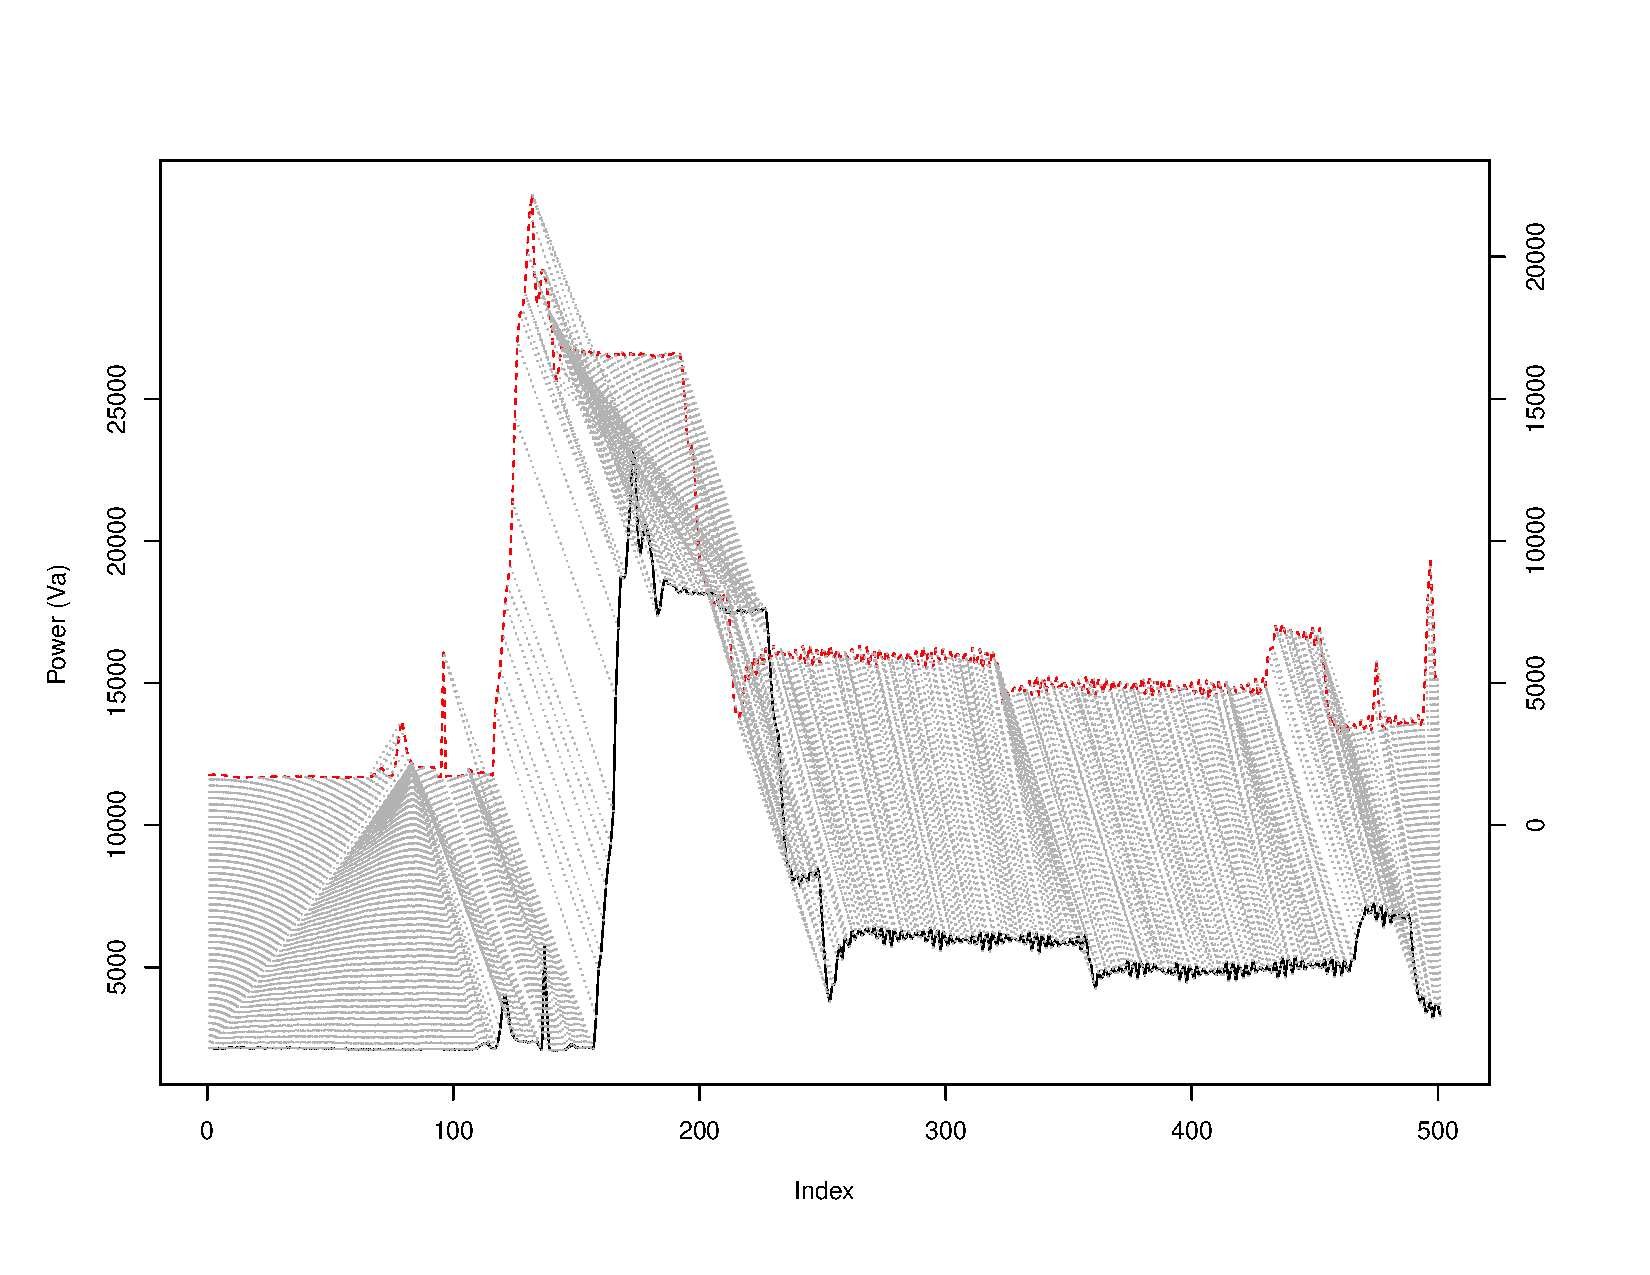
\includegraphics[width=14cm,height=11cm]{Images/dtw_match}
\par\end{centering}

\caption{Mapping of two time streams using DTW\label{fig:dtw fig}}


\end{figure}


As we can see in Fig \ref{fig:dtw fig}, even if we have a time shift
and small variations in data, the DTW algorithm maps significant features
appropriately. This robustness is a result of the warping along time
direction allowed. One can also limit the amount of warping permissible
so that we can ensure that only physically possible cases are deemed
similar. The distance between two sequences being compared is found
has sum of distances (euclidean, manhattan, etc) between these mapped
points.


\subsection{Extracting input from power consumption pattern}

\noindent \begin{center}
Now we have the start and end times for 300 producing cycles and we
can use this data to get power consumption patterns for each individual
part and use it as necessary. However, we can't use these patterns
directly as inputs for any machine llearning algorithm as it has many
inherent problems. The main reason being that small time offsets in
the time series data could throw off the result by a large amount.
So we basically needed to process our power pattern to extract more
stable information from it. However in the process of making it stable,
we also have to make sure that we don\textquoteright{}t lose the individuality
of the pattern as we depend on this individual character for our quality
reading. We resolved this using two methods:-
\par\end{center}
\begin{enumerate}
\item Scalar extractions from pattern.
\item Cycle splitting.
\end{enumerate}

\subsubsection{Scalar extractions from splitting}

Here we extract from our cycle a set of scalars which are stable and
do not get affected due to small changes like minor time scaling,
peaks,etc. These scalars could be mean, standard deviation, DTW distance,
median, mode, amplitude, etc. However, as pointed out earlier, using
these scalars alone would render many cycles to be same as we are
wasting a lot of information. So we use, not one, but a combination
of these scalars as now we get more options of variability thus giving
us our desired result of stable and unique inputs.


\subsubsection{Cycle splitting}

This is a much more important process and increases the effectiveness
of scalar extraction. What we essentially do cut the cycle into a
number of parts using different methods (which will be discussed later)
and apply the scalar extraction for each segment. So now we increase
our number of inputs and also increase the individuality of each input
in a stable way. 

Much more importantly, when we later analyze our results, we can actually
pinpoint which segments of the cycle are primarily responsible for
the quality parameter being measured (in our case, Ra). This kind
of information can prove to be really useful as now we can know what
part of the cycle is primarily responsible for which quality parameter.
This can in turn help us detecting tool damages when we observe a
deviation in certain quality parameter. Splitting the cycle gives
us one more important advantage. Now we can calculate the quality
metric of a cycle by including one split at a time, into our input
set, sequentially. This can be really helpful in predicting parameter
qualities before the machining is over and thus can help us in taking
corrective action.

We primarily employed four different methods to split cycles. They
were:-%
\begin{comment}
Insert figures
\end{comment}

\begin{enumerate}
\item \textbf{Uniform splitting}: As the name suggests, we split the cycle
into equally sized sections. The number of parts would depend on how
much accuracy we want and how much computation cost we can afford
(Fig \ref{fig:Uniform-splitting}).
\begin{figure}[!tph]
\noindent \centering{}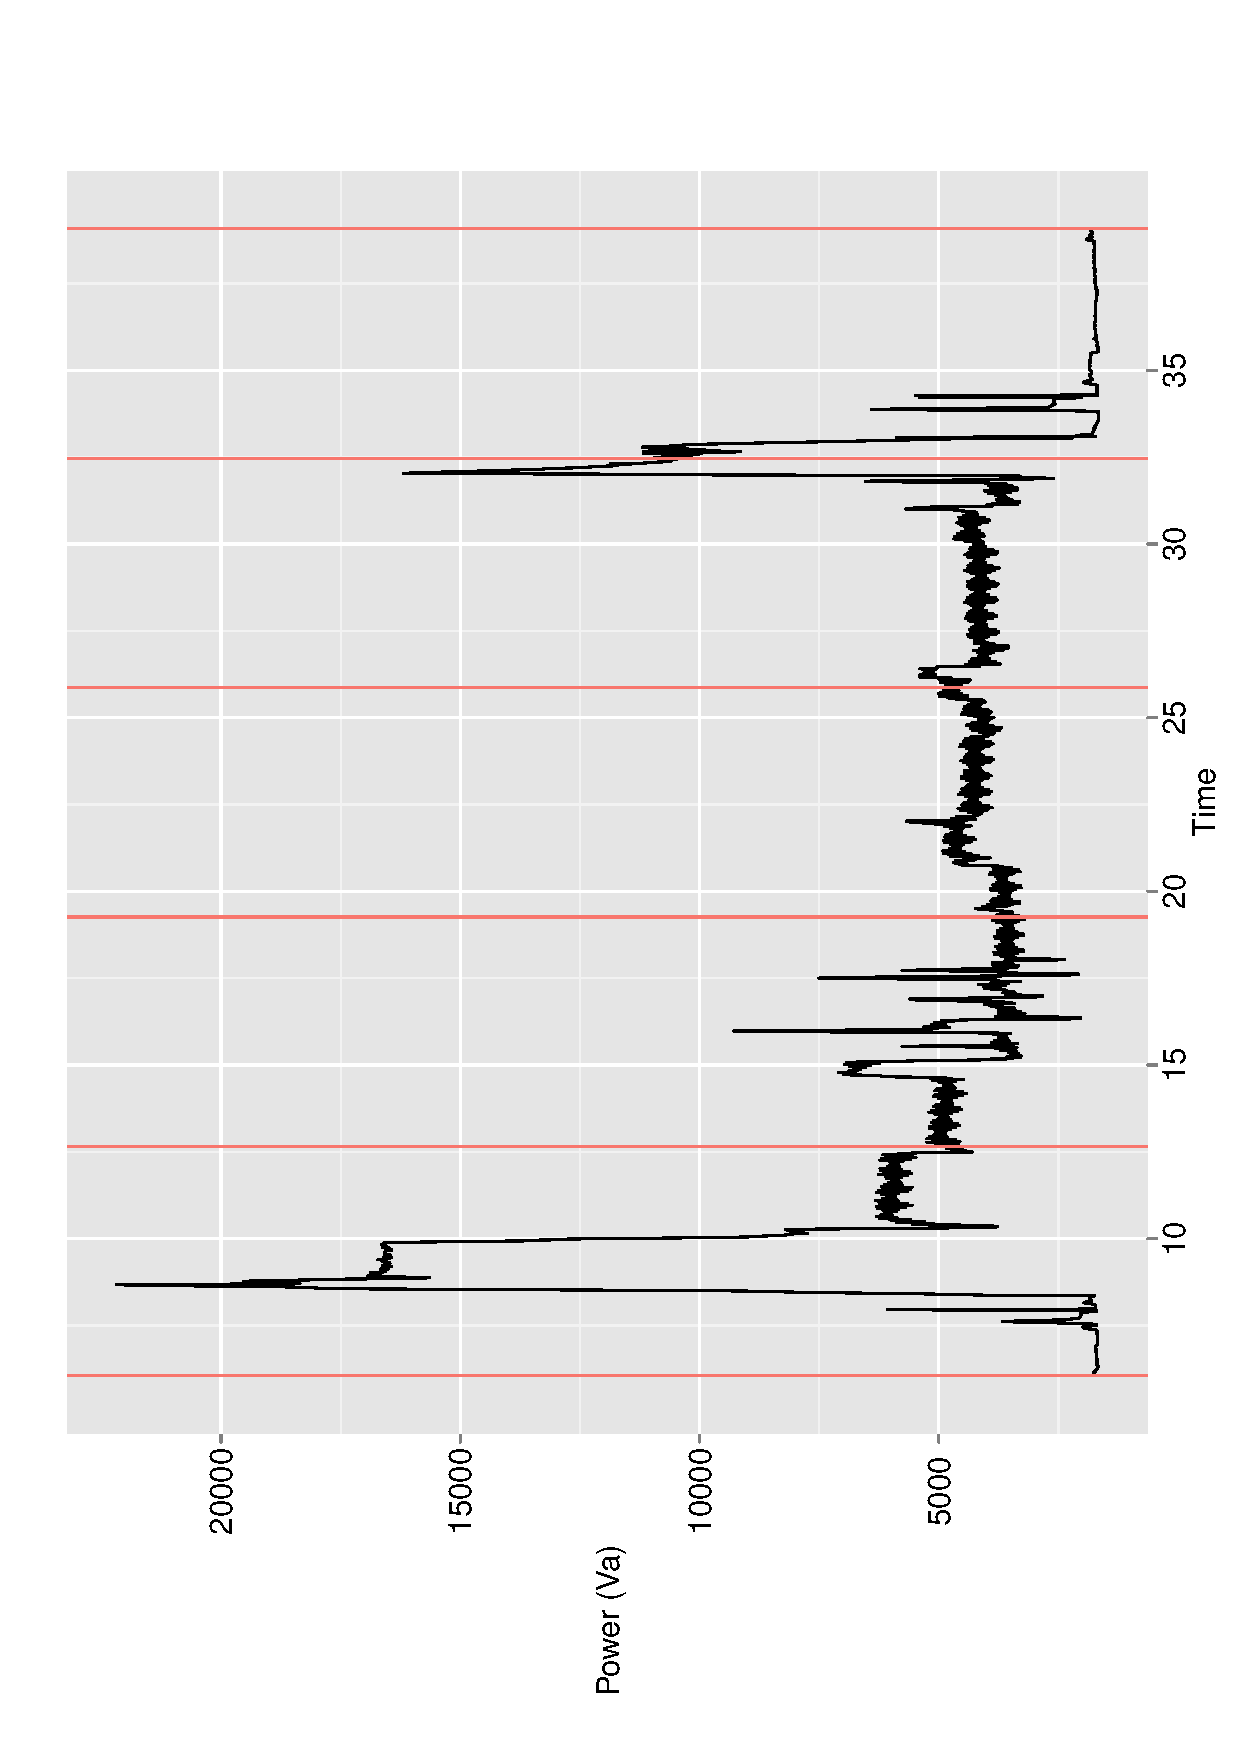
\includegraphics[width=14cm,height=8cm]{Images/uniform_split}\caption{Uniform splitting (5 sections)\label{fig:Uniform-splitting}}
\end{figure}

\item \textbf{Forward feedback splitting}: This is a process in which we
make a cut by splitting a section into two equal halves and decide
whether we keep that cut by checking if the amount of improvement
we get is significant enough. It is slightly biased to create more
cuts in the beginning of the cycle as we move on to the former section
after a cut has been made and move to the next section only if no
more cuts can be made in the former one (Fig \ref{fig:Forward-feedback-splitting}).
\begin{figure}[!tph]
\noindent \begin{centering}
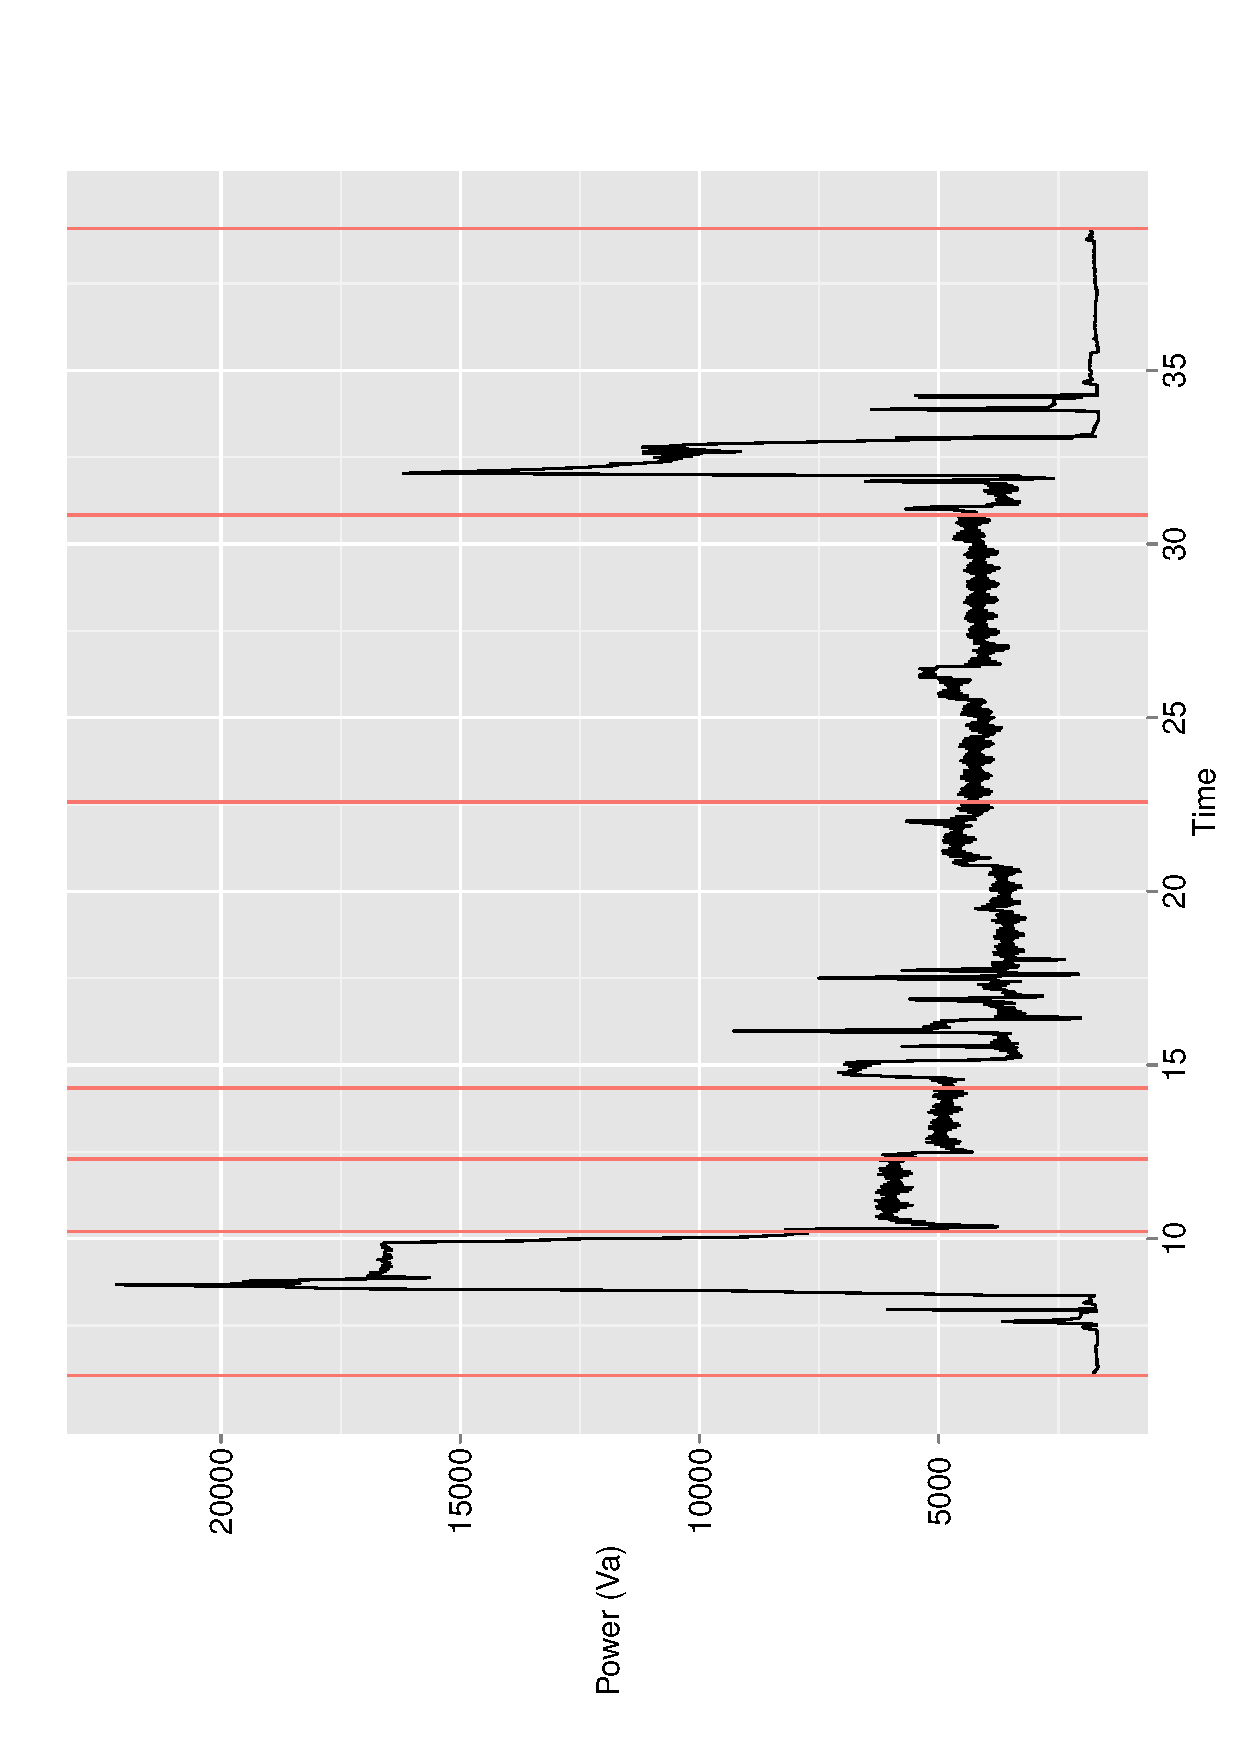
\includegraphics[width=14cm,height=8cm]{Images/forward_split}
\par\end{centering}

\noindent \centering{}\caption{Forward feedback splitting\label{fig:Forward-feedback-splitting}}
\end{figure}

\item \textbf{Reverse feedback splitting}: This is almost like the Forward
Feedback Splitting but instead of biasing cuts to the start, this
one biases cuts to the end (\ref{fig:Reverse-Feedback-splitting}).
\begin{figure}[!tph]
\noindent \begin{centering}
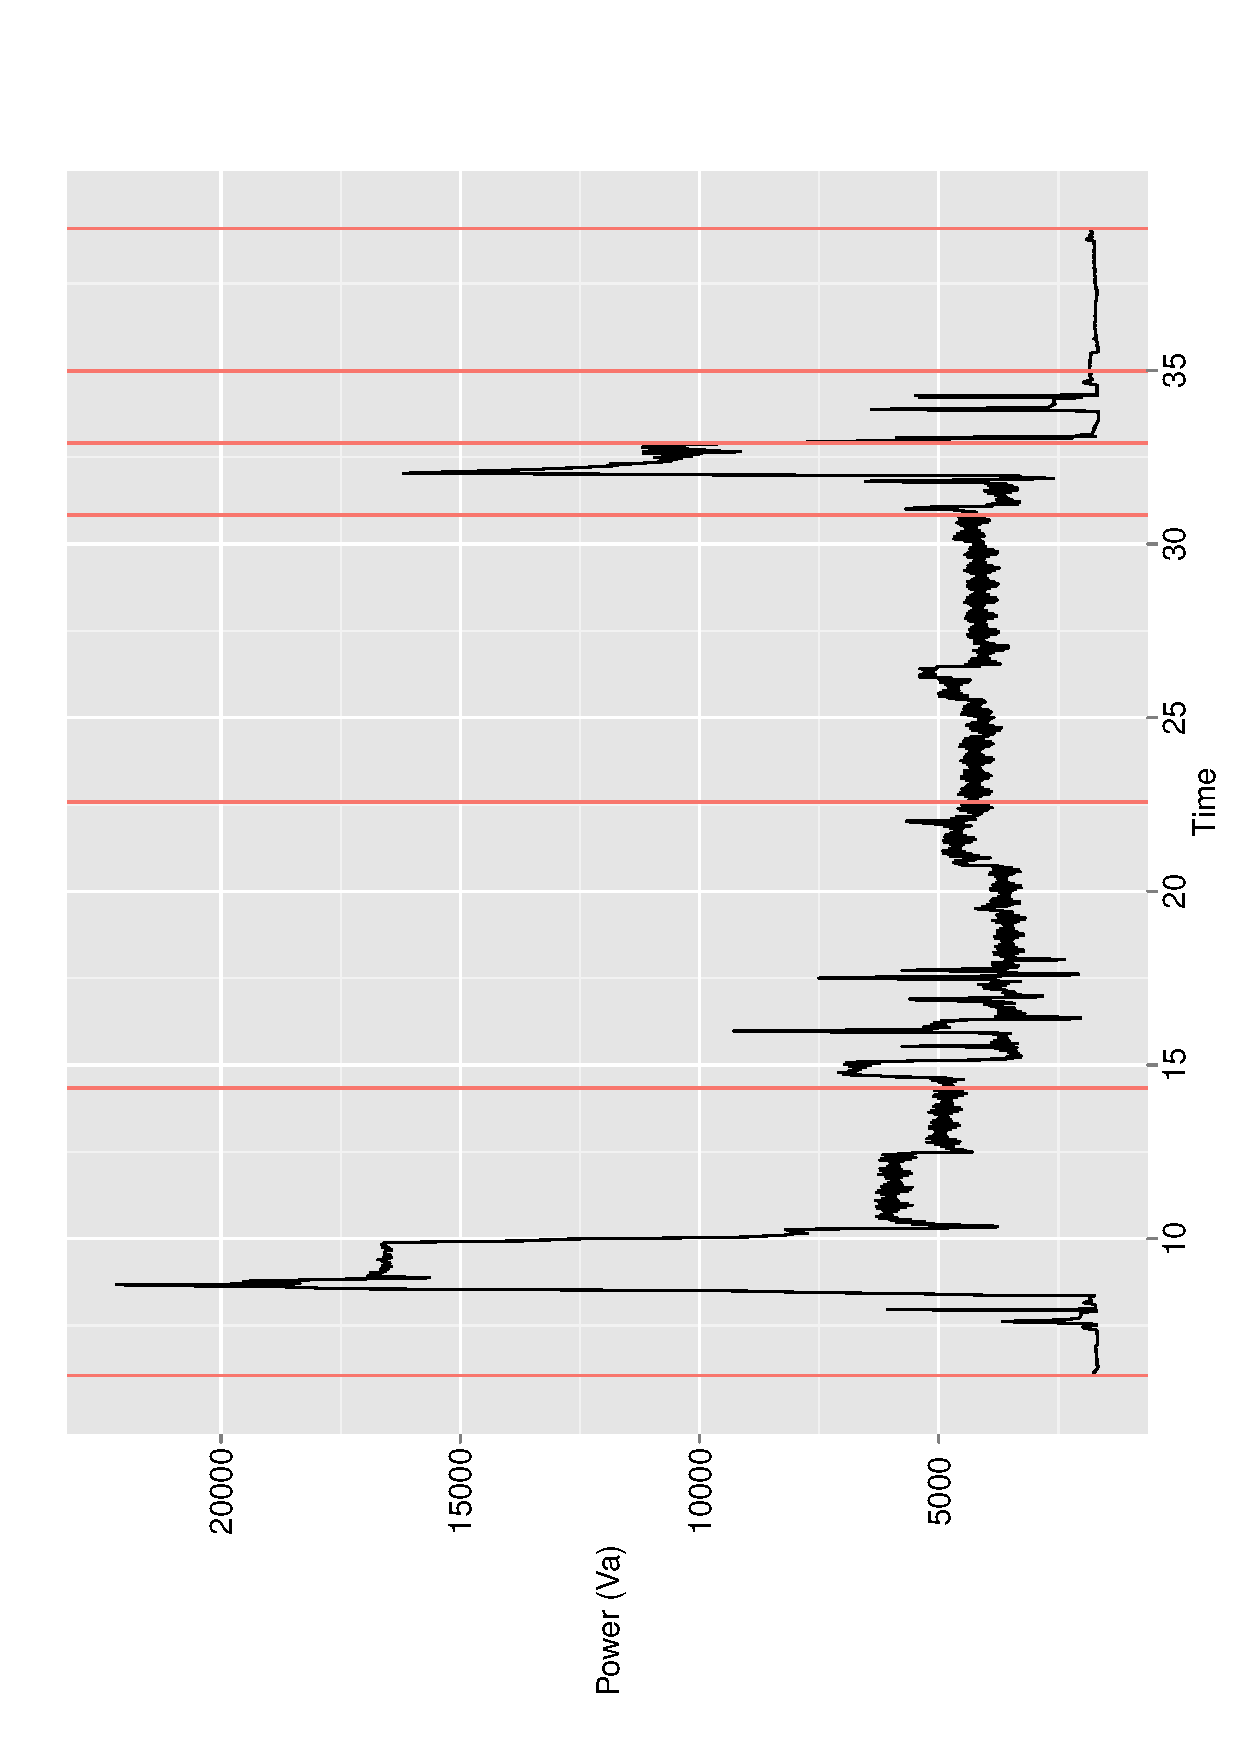
\includegraphics[width=14cm,height=8cm]{Images/reverse_split}
\par\end{centering}

\noindent \centering{}\caption{Reverse Feedback splitting\label{fig:Reverse-Feedback-splitting}}
\end{figure}

\item \textbf{Phase dependent splits}: These are cuts which signify a change
in process in the machining. Theoretically, these should be the most
optimum cuts as they point towards specific process. However, finding
them out autonomously can be tricky if wanted for all situations thus
these cuts have to be entered manually (Fig \ref{fig:Phase-dependent-split}).
\begin{figure}[!tph]
\noindent \begin{centering}
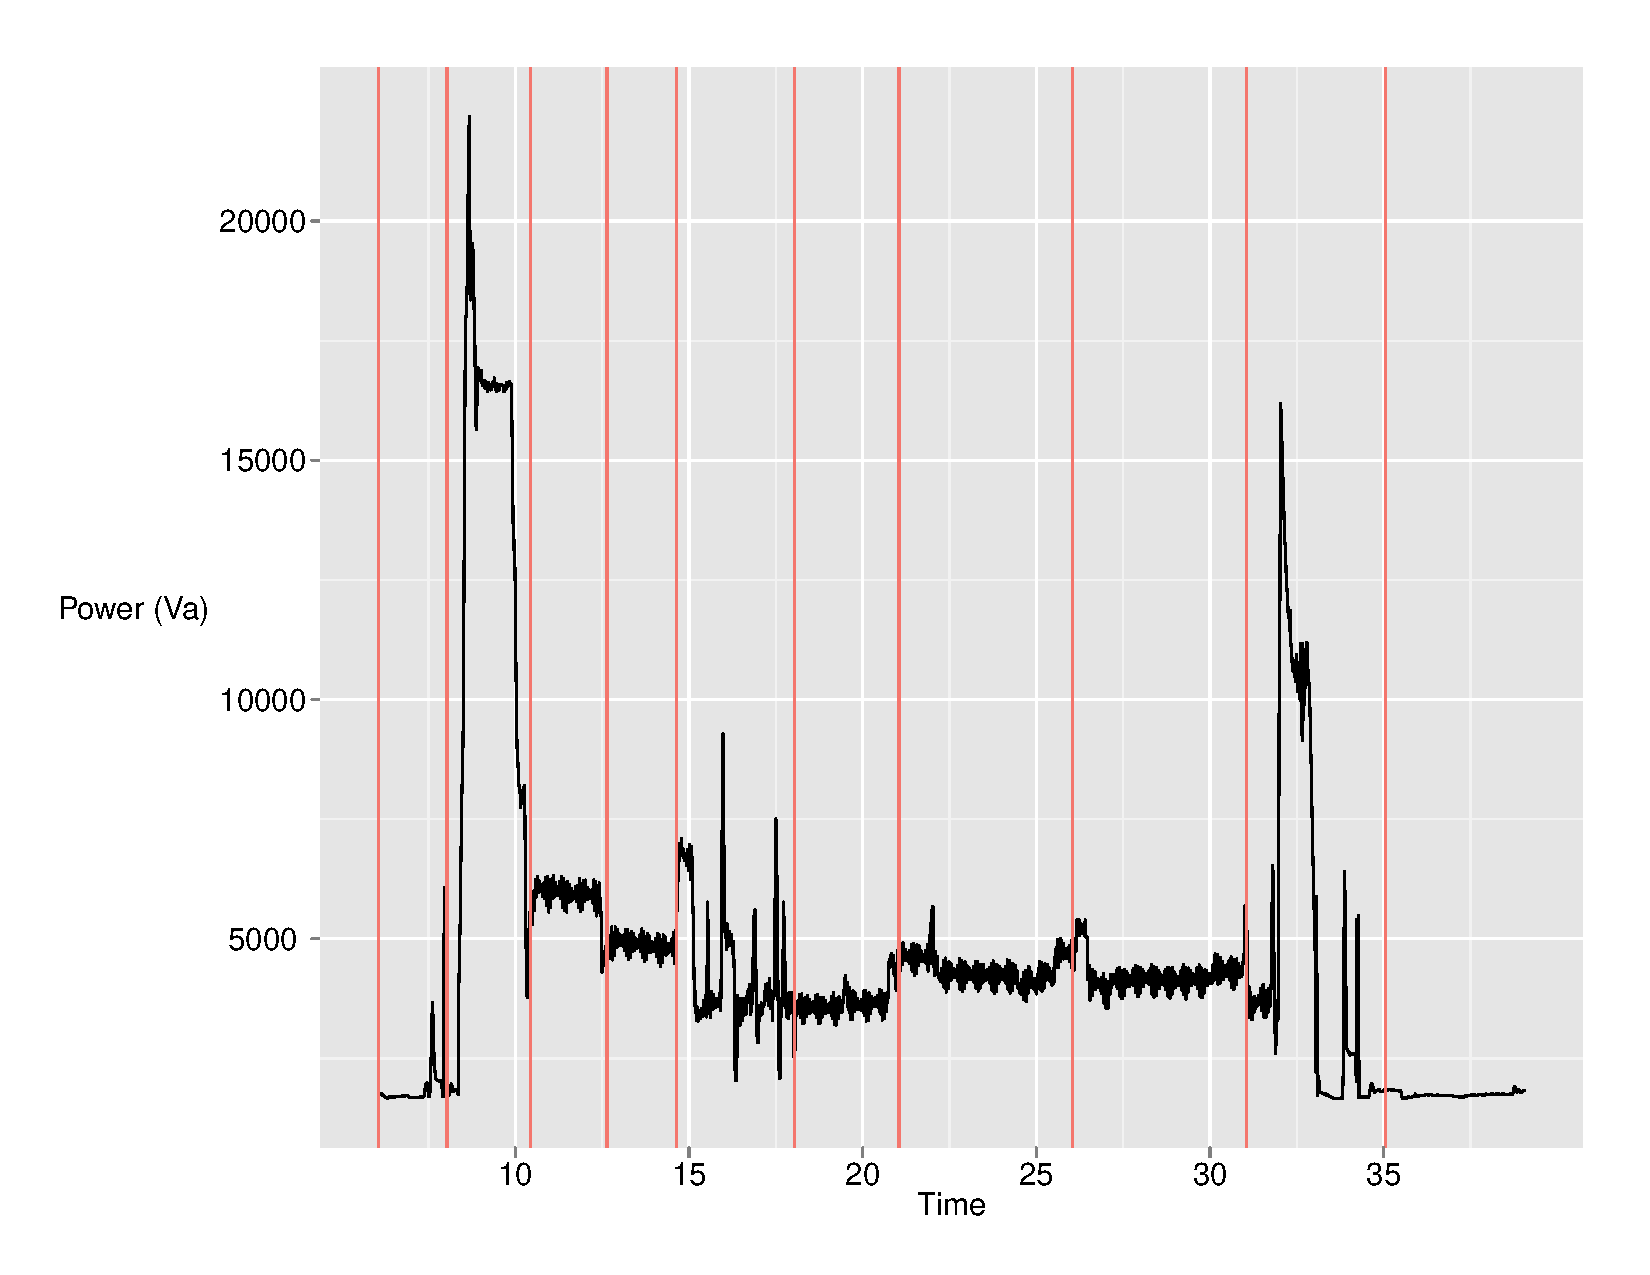
\includegraphics[width=14cm,height=8cm]{Images/manual_split}
\par\end{centering}

\noindent \centering{}\caption{Phase dependent split\label{fig:Phase-dependent-split}}
\end{figure}

\end{enumerate}
Now, after splitting the cycle appropriately and using scalar extraction
for each split, we have a bunch of variables for a cycle which we
will later use to get a wider set of data.


\subsection{Model Selection}

There are a plethora%
\begin{comment}
CHECK IF THERE ACTUALLY ARE A PLETHORA OF METHODS
\end{comment}
{} of machine learning algorithms which we could use to establish a
relation between our input and output. We decided to try the very
simple models and thus decided to use \emph{Polynomial Regression.}
However, as our number of variables were bound to be high, we decided
to keep the model complexity to a minimum and thus decided to go forward
with \emph{Regularised Polynomial Regression.}


\subsubsection{Regularised Regression}

Say we try to create a linear relation between input variables$x_{1},x_{2},x_{3}....,x_{n}$and
output variable $y.$As it is linear, we can assume our equation to
be
\begin{equation}
y=a_{0+}a_{1}x_{1}+a_{2}x_{2}+a_{3}x_{3}.......+a_{n}x_{n}\label{eq:regul 1}
\end{equation}


Where $a_{1},a_{2},a_{3}.......a_{n}$ are the coefficients which
we have to find. 

Let us define input variable $\mathbf{X}$ and $\mathbf{A}$ as 
\begin{equation}
\mathbf{X_{i}=}(x_{1,}^{i}x_{2}^{i},x_{3}^{i},......,x_{n}^{i})\label{eq:regul 2}
\end{equation}


\begin{equation}
\mathbf{A}=(a_{1},a_{2},a_{3},.....,a_{n})\label{eq:regul 3}
\end{equation}


where $x_{j}^{i}$ is the $i^{th}$ instance of the $j^{th}$ variable.
Thus, we get
\begin{equation}
y_{i}=a_{0+}a_{1}x_{1}^{i}+a_{2}x_{2}^{i}+a_{3}x_{3}^{i}.......+a_{n}x_{n}^{i}\label{eq:regul 4}
\end{equation}


Now, say we have the $p$ values of $\mathbf{X}_{i}$and its corresponding
output which we denote by $\mathbf{Y}_{i}$. So to find the best approximation
of $\mathbf{A}$, we minimize the difference between $\mathbf{Y}_{i}$and
$y_{i}$. Let our final coefficients' set be $\mathbf{A}_{LS}$. Using
least square method, we get
\begin{equation}
\mathbf{A_{LS}}=\arg\min_{\mathbf{A}}(\sum_{i=1}^{p}(y_{i}-\mathbf{Y_{i}})^{2})\label{eq:regul 5}
\end{equation}


which can be re-written as 
\begin{equation}
\mathbf{A_{LS}=\arg\min}(\sum_{i=1}^{p}(\mathbf{A}^{T}\mathbf{X_{i}}-\mathbf{Y_{i}})^{2})\label{eq:regul 6}
\end{equation}


Thus as a result of linear regression, we finally get
\begin{equation}
y=\mathbf{A_{LS}^{T}X}\label{eq:regul 7}
\end{equation}


when $x_{j}$ are polynomial forms of each other, this is called polynomial
regression.

However, when the number of variables are high, i:e, when $n$ is
large, we tend to get highly complex models with high values of $a_{i}$
which tend to overfit $y$ as a function of $\mathbf{X}$. To remedy
this, we include a regularization parameter $\lambda$, such that,
$\lambda>0$ and 
\begin{equation}
\mathbf{A_{LS}=\arg\min}(\sum_{i=1}^{p}(\mathbf{A}^{T}\mathbf{X_{i}}-\mathbf{Y_{i}})^{2}+\lambda\sum_{j=1}^{n}a_{j}^{2})\label{eq:regul 8}
\end{equation}


Thus, now we can control, via $\lambda$, how complex a system we
want. Too high a $\lambda$ gives us an overfit solution while too
low a $\lambda$ gives us an underfit one.


\subsection{Model Creation}

To implement \emph{Regularised Polynomial Regression, }we first need
to use our present variable set (which we got after extracting scalars
from split sections of a cycle) to form polynomial variables. Firstly
we divide our 300 cycles into two sets, a \emph{training set} and
a \emph{testing set}. each cycle is assigned to one of these sets
randomly and the ratio between the number of elements in the two sets
can be decided by us. we chose a 1:1 ratio. Now, in the training set,
for each variable (scalar from a split section), we have 150 other
instances of the same corresponding to 150 cycles. This gives us a
vector of that corresponding variable.This way we have a vector corresponding
to all the variables. These vectors will be used to create the polynomial
variables which will eventually be used as inputs into the \emph{Regularised
Linear Regression. }This we do in two ways:-
\begin{enumerate}
\item \textbf{Orthogonal polynomials- }We create new vectors which are orthonormal
to each of the vector of variables we have. The degree of these orthogonal
variables were varied to see which would yield reasonable results.%
\begin{comment}
ADD ORTHOGONAL POLYNOMIAL EQUATION IF NEEDED
\end{comment}

\item \textbf{Mixed polynomials-} Here we create new vectors using the old
variable vectors (denoted as $x_{1},x_{2},x_{3}....,x_{n}$) which
can be shown asllll
\begin{equation}
x_{new}(i_{1},i_{2},i_{3},.....i_{n})=\prod_{j=1}^{n}x_{j}^{i_{j}};\label{eq:mixed_poly_1}
\end{equation}

\end{enumerate}
where

\begin{equation}
i_{1},i_{2},i_{3}....i_{n}=0,1,2,3,4.....;\label{eq:mixed_poly_2}
\end{equation}


and

\begin{equation}
\sum_{j=1}^{n}i_{j}<=p;\label{eq:mixed_poly_3}
\end{equation}


Where $p$ is the maximum degree which we vary to get optimum results.
As expected, we get more number of variables using this method instead
of the orthogonal polynomials one. However, it helps us know if there
are any meaningful interactions within the variables.

Now that we have our input vectors' set created, we just a \emph{Regularised
Linear Regression }to get a list of possible relations between our
input quality. In the next section we discuss how we select the right
parameters from this given list.


\subsection{Parameter comparison and selection}

The output of the \emph{regularised polynomial regression }is a list
of solutions. Each solution contains a collection of coefficients
which we use for a weighted summation of our newly calculated variable
vectors. To compare between these various solutions, we use them and
predict quality parameter values for our test set and then we compare
these predicted values against our polynomial fit values (from \ref{sub:Getting-Quality-data}
) and find out the \emph{root mean square error(RMSE), }where we assume
that the polynomial fit values are the true values. We use this \emph{RMSE
}as a metric to compare between the solutions and pick the solution
with minimum \emph{RMSE.}


\section{Results}

\appendix

\section{Appendix name}

Appendix, only when needed.


\section*{-----------------}

You can use either Bib\TeX{}:

\bibliographystyle{elsarticle-harv}
\addcontentsline{toc}{section}{\refname}\bibliography{../examples/biblioExample}



\section*{---------------------}

\noindent Or plain bibliography:
\begin{thebibliography}{References}
\bibitem{key-1}Frank Mittelbach and Michel Goossens: \emph{The \LaTeX{}
Companion Second Edition.} Addison-Wesley, 2004.

\bibitem{key-2}Scott Pakin. The comprehensive \LaTeX{} symbol list,
2005.\end{thebibliography}

\end{document}
